\documentclass[12pt]{article}



\usepackage{amsmath}
\usepackage[margin = 2cm]{geometry}
\usepackage{tikz}
\usepackage{float}
\usepackage{listings}
\usepackage{xcolor}



\lstdefinestyle{console}{
    backgroundcolor=\color{gray!10},
    basicstyle=\ttfamily\small,
    frame=single,
    breaklines=true
}



\begin{document}


%%%%%%%%%%%%%%%%%%%%%%%%%%%%%%%%%%%%%%%%%%%%%%%%%%%%%%%%%%%%
\section{Algorithms and Cryptography Utilities}
%%%%%%%%%%%%%%%%%%%%%%%%%%%%%%%%%%%%%%%%%%%%%%%%%%%%%%%%%%%%

\subsection{RSA Key Generation: generateRSAKeyPair()}

\subsubsection{Purpose}

The RSA key generation algorithm is responsible for creating a public-private
key pair for each user. The public key can be distributed openly, while the
private key must remain secret.

\subsubsection{Mathematical Foundation}

Two distinct prime numbers $p$ and $q$ are selected.

The RSA modulus is computed as

\begin{equation}
n = pq.
\end{equation}

The Euler totient function is then calculated:

\begin{equation}
\phi(n) = (p-1)(q-1).
\end{equation}

A public exponent $e$ is selected such that

\begin{equation}
gcd(e,\phi(n)) = 1.
\end{equation}

Finally, the private exponent $d$ is computed as the modular inverse of $e$:

\begin{equation}
d \equiv e^{-1} \pmod{\phi(n)}.
\end{equation}

\subsubsection{Implementation}

The method \texttt{generateRSAKeyPair()} performs the following steps:

\begin{enumerate}
\item Select two distinct prime numbers from the predefined prime list.
\item Compute $n=pq$.
\item Compute $\phi(n)$.
\item Select the public exponent $e$.
\item Verify that $e$ and $\phi(n)$ are relatively prime.
\item Compute $d$ using the modular inverse algorithm.
\item Return the generated key pair.
\end{enumerate}

\subsubsection{Role in the Project}

RSA keys are used for digital signatures and certificate generation.

%%%%%%%%%%%%%%%%%%%%%%%%%%%%%%%%%%%%%%%%%%%%%%%%%%%%%%%%%%%%

\subsection{Euclidean Algorithm: gcd(long a, long b)}

\subsubsection{Purpose}

The Greatest Common Divisor (GCD) algorithm is used to verify that the public
exponent $e$ is relatively prime to $\phi(n)$.

\subsubsection{Mathematical Foundation}

The Euclidean Algorithm is based on the identity

\begin{equation}
gcd(a,b) = gcd(b,a \bmod b).
\end{equation}

The procedure continues until the second argument becomes zero.

\subsubsection{Implementation}

The method repeatedly computes the remainder

\begin{equation}
r = a \bmod b,
\end{equation}

and updates the variables until

\begin{equation}
b = 0.
\end{equation}

The final value of $a$ is returned as the greatest common divisor.

%%%%%%%%%%%%%%%%%%%%%%%%%%%%%%%%%%%%%%%%%%%%%%%%%%%%%%%%%%%%

\subsection{Fast Modular Exponentiation: \\
modPower(long base, long exp, long mod)}

\subsubsection{Purpose}

RSA signatures and Diffie-Hellman key exchange require efficient computation
of modular powers of the form

\begin{equation}
a^b \bmod n.
\end{equation}

\subsubsection{Mathematical Foundation}

The algorithm uses the square-and-multiply technique.

Instead of performing $b$ multiplications, the exponent is processed bit by
bit. Repeated squaring is used to generate higher powers efficiently.

For example,

\begin{equation}
a^{13}=a^{8}\times a^{4}\times a^{1}
\end{equation}

since

\begin{equation}
13=(1101)_2.
\end{equation}

\subsubsection{Implementation}

The algorithm performs the following operations:

\begin{enumerate}
\item Initialize the result to 1.
\item While the exponent is non-zero:
\begin{enumerate}
\item If the least significant bit is 1, multiply the result by the current base.
\item Square the base.
\item Shift the exponent one bit to the right.
\end{enumerate}
\item Return the final result.
\end{enumerate}

%%%%%%%%%%%%%%%%%%%%%%%%%%%%%%%%%%%%%%%%%%%%%%%%%%%%%%%%%%%%

\subsection{Modular Inverse Algorithm: modInverse(long a, long m)}

\subsubsection{Purpose}

The modular inverse algorithm computes the RSA private exponent $d$.

\subsubsection{Mathematical Foundation}

The objective is to find $d$ satisfying

\begin{equation}
ed \equiv 1 \pmod{\phi(n)}.
\end{equation}

The Extended Euclidean Algorithm computes integers $x$ and $y$ such that

\begin{equation}
ax+my=gcd(a,m).
\end{equation}

Since

\begin{equation}
gcd(e,\phi(n))=1,
\end{equation}

we obtain

\begin{equation}
ex+\phi(n)y=1.
\end{equation}

Therefore,

\begin{equation}
x=e^{-1}\pmod{\phi(n)},
\end{equation}

which becomes the RSA private exponent.

\subsubsection{Implementation}

The method iteratively updates coefficients until the modular inverse is
obtained. If the result is negative, it is converted to the equivalent positive
value.

%%%%%%%%%%%%%%%%%%%%%%%%%%%%%%%%%%%%%%%%%%%%%%%%%%%%%%%%%%%%

\subsection{XOR-Based Hash Function: simpleHash(String data)}

\subsubsection{Purpose}

The hash function generates a compact representation of a message before it is
digitally signed.

\subsubsection{Mathematical Foundation}

Given message bytes

\begin{equation}
b_1,b_2,\ldots,b_n
\end{equation}

the hash value is computed as

\begin{equation}
H=b_1 \oplus b_2 \oplus \cdots \oplus b_n
\end{equation}

where $\oplus$ denotes the XOR operation.

\subsubsection{Implementation}

The input string is converted into bytes. Each byte is then XORed with the
current hash value until a single 8-bit result remains.

%%%%%%%%%%%%%%%%%%%%%%%%%%%%%%%%%%%%%%%%%%%%%%%%%%%%%%%%%%%%

\subsection{RSA Digital Signature Generation: \\
sign(String data, RSAKeyPair keys)}

\subsubsection{Purpose}

Digital signatures provide authentication, integrity, and non-repudiation.

\subsubsection{Mathematical Foundation}

First, the message hash is computed:

\begin{equation}
h = H(m).
\end{equation}

The signature is then generated using the RSA private key:

\begin{equation}
S = h^d \bmod n.
\end{equation}

\subsubsection{Implementation}

The method performs two operations:

\begin{enumerate}
\item Compute the message hash.
\item Apply modular exponentiation using the RSA private exponent.
\end{enumerate}

\subsubsection{Role in the Project}

Digital signatures are used by the Certificate Authority (CA) and by users
during the authenticated Diffie-Hellman protocol.

%%%%%%%%%%%%%%%%%%%%%%%%%%%%%%%%%%%%%%%%%%%%%%%%%%%%%%%%%%%%

\subsection{RSA Digital Signature Verification: \\ 
verify(String data, long signature, long e, long n)}

\subsubsection{Purpose}

Signature verification confirms both message integrity and sender authenticity.

\subsubsection{Mathematical Foundation}

The verifier computes

\begin{equation}
h_1 = H(m),
\end{equation}

and recovers

\begin{equation}
h_2 = S^e \bmod n.
\end{equation}

If

\begin{equation}
h_1 = h_2
\end{equation}

the signature is considered valid.

\subsubsection{Implementation}

The verification process consists of:

\begin{enumerate}
\item Recomputing the hash of the received data.
\item Recovering the signed hash using the public key.
\item Comparing the two values.
\end{enumerate}

\subsubsection{Security Interpretation}

A successful verification indicates that:

\begin{itemize}
\item the message has not been modified;
\item the signature was generated by the holder of the corresponding private key.
\end{itemize}
\newpage

%%%%%%%%%%%%%%%%%%%%%%%%%%%%%%%%%%%%%%%%%%%%%%%%%%%%%%%%%
%%%%%%%%%%%%%%%%%%%%%%%%%%%%%%%%%%%%%%%%%%%%%%%%%%%%%%%%%
\section{Certificate Authority and Certificate Management}

%%%%%%%%%%%%%%%%%%%%%%%%%%%%%%%%%%%%%%%%%%%%%%%%%%%%%%%%%%%%

\subsection{Certificate Authority (CA)}

\subsubsection{Purpose}

A Certificate Authority (CA) is a trusted entity responsible for binding a
user's identity to a public key. The CA issues digitally signed certificates
that allow other users to verify the authenticity of public keys.

\subsubsection{Role in the Project}

In this project, the CA performs the following tasks:

\begin{enumerate}
\item Generates its own RSA key pair.
\item Issues certificates for users.
\item Signs certificate contents using its private key.
\item Verifies issued certificates using its public key.
\end{enumerate}

All participants trust the CA's public key. Consequently, any certificate
successfully verified using this public key is considered authentic.

%%%%%%%%%%%%%%%%%%%%%%%%%%%%%%%%%%%%%%%%%%%%%%%%%%%%%%%%%%%%

\subsection{Certificate Issuance Algorithm: 
issueCertificate(User user)}

\subsubsection{Purpose}

The certificate issuance algorithm creates a digital certificate that binds a
user's identity to their RSA public key.

This allows other users to verify that a public key genuinely belongs to the
claimed owner.

\subsubsection{Certificate Structure}

Each certificate contains:

\begin{equation}
Certificate =
(ID,n,e,Signature),
\end{equation}

where:

\begin{itemize}
\item $ID$ is the user identifier.
\item $n$ is the RSA modulus.
\item $e$ is the RSA public exponent.
\item $Signature$ is the CA's digital signature.
\end{itemize}

\subsubsection{Mathematical Foundation}

The CA first constructs the certificate data:

\begin{equation}
String = ID \; || \; n \; || \; e,
\end{equation}

where $||$ denotes concatenation.

The hash of the certificate data (string) is then computed:

\begin{equation}
h = H(String).
\end{equation}

The CA signs the hash using its RSA private key:

\begin{equation}
Signature = h^{d_{CA}} \bmod n_{CA}
\end{equation}

The resulting signature is embedded within the certificate.

\subsubsection{Implementation}

The method \texttt{issueCertificate()} performs the following steps:

\begin{enumerate}
\item Retrieve the user's identifier.
\item Retrieve the user's RSA public key components $(n,e)$.
\item Concatenate the fields into a single string.
\item Generate a digital signature using the CA's private key.
\item Create and return a certificate object.
\end{enumerate}

\subsubsection{Security Contribution}

The certificate ensures that the public key cannot be replaced without
invalidating the CA's signature. Any modification of the certificate contents
causes signature verification to fail.

%%%%%%%%%%%%%%%%%%%%%%%%%%%%%%%%%%%%%%%%%%%%%%%%%%%%%%%%%%%%

\subsection{Certificate Verification Algorithm: \\
verifyCertificate(Certificate certificate)}

\subsubsection{Purpose}

Certificate verification determines whether a certificate was genuinely issued
by the trusted Certificate Authority and whether its contents have been altered.

\subsubsection{Mathematical Foundation}

The verifier reconstructs the certificate data:

\begin{equation}
String = ID \; || \; n \; || \; e,
\end{equation}

and computes:

\begin{equation}
h_1 = H(String).
\end{equation}

The signed hash is then recovered using the CA's public key:

\begin{equation}
h_2 = Signature^{e_{CA}} \bmod n_{CA}.
\end{equation}

If

\begin{equation}
h_1 = h_2
\end{equation}

the certificate is considered valid.

\subsubsection{Implementation}

The method \texttt{verifyCertificate()} performs the following operations:

\begin{enumerate}
\item Extract the certificate fields.
\item Reconstruct the original certificate data.
\item Compute the expected hash.
\item Recover the signed hash using the CA public key.
\item Compare the two values.
\end{enumerate}

A certificate is accepted only if both hashes are identical.

\subsubsection{Security Interpretation}

A successful verification guarantees that:

\begin{itemize}
\item the certificate was issued by the trusted CA;
\item the certificate contents have not been modified;
\item the contained public key belongs to the claimed user.
\end{itemize}

%%%%%%%%%%%%%%%%%%%%%%%%%%%%%%%%%%%%%%%%%%%%%%%%%%%%%%%%%%%%

\subsection{Trust Model of the PKI}

The security of the entire Public Key Infrastructure depends on the trust placed
in the Certificate Authority.

All users trust the CA's public key and use it to verify certificates.
Therefore, trust in a user's public key is derived from trust in the CA.

This trust relationship can be summarized as:

\begin{equation}
User \rightarrow Certificate \rightarrow CA
\end{equation}

If the CA's signature is valid, the user's public key is accepted as authentic.




%%%%%%%%%%%%%%%%%%%%%%%%%%%%%%%%%%%%%%%%%%%%%
%%%%%%%%%%%%%%%%%%%%%%%%%%%%%%%%%%%%%%%%%%%%%

\newpage
%%%%%%%%%%%%%%%%%%%%%%%%%%%%%%%%%%%%%%%%%%%%%%%%%%%%%%%%%%%%
\section{Authenticated Diffie-Hellman Key Exchange}
%%%%%%%%%%%%%%%%%%%%%%%%%%%%%%%%%%%%%%%%%%%%%%%%%%%%%%%%%%%%

\subsection{Purpose}

The objective of the Diffie--Hellman protocol is to allow two parties to
establish a common secret key over an insecure communication channel.

A fundamental limitation of the basic Diffie--Hellman protocol is its
vulnerability to Man-in-the-Middle (MITM) attacks. An attacker can intercept
and replace public values exchanged between the two parties, thereby creating
independent keys with each victim.

To address this weakness, the implementation combines Diffie--Hellman with
digital certificates and RSA signatures. As a result, both confidentiality and
authentication are achieved.

%%%%%%%%%%%%%%%%%%%%%%%%%%%%%%%%%%%%%%%%%%%%%%%%%%%%%%%%%%%%

\subsection{Public Parameters}

The protocol uses two public constants:

\begin{equation}
p = 65521
\end{equation}

\begin{equation}
g = 11,
\end{equation}

where:

\begin{itemize}
\item $p$ is a large prime modulus,
\item $g$ is a generator of the multiplicative group modulo $p$.
\end{itemize}

These values are publicly known to all participants.

%%%%%%%%%%%%%%%%%%%%%%%%%%%%%%%%%%%%%%%%%%%%%%%%%%%%%%%%%%%%

\subsection{Certificate Validation Phase}

\subsubsection{Purpose}

Before any key exchange takes place, each participant must verify the
authenticity of the other participant's certificate.

This step ensures that the public keys used during authentication genuinely
belong to the claimed users.

\subsubsection{Implementation}

The protocol begins by verifying both certificates:

\begin{verbatim}
verifyCertificate(A)
verifyCertificate(B).
\end{verbatim}

If either certificate fails verification, the protocol terminates immediately.

\subsubsection{Security Contribution}

Certificate validation prevents attackers from introducing fraudulent public
keys into the protocol.

Without this step, authentication would be meaningless because participants
could not trust the public keys they receive.

%%%%%%%%%%%%%%%%%%%%%%%%%%%%%%%%%%%%%%%%%%%%%%%%%%%%%%%%%%%%

\subsection{Private Key Generation}

\subsubsection{Purpose}

Each participant generates a secret Diffie-Hellman exponent.

These values remain private and are never transmitted through the network.

\subsubsection{Mathematical Foundation}

Alice selects:

\begin{equation}
a \in [2,p-1].
\end{equation}

Bob selects:

\begin{equation}
b \in [2,p-1].
\end{equation}

Both values are generated randomly.

\subsubsection{Implementation}

The implementation generates:

\begin{verbatim}
a = 2 + random.nextInt(65519)
b = 2 + random.nextInt(65519),
\end{verbatim}

which ensures that both values lie in the interval

\begin{equation}
2 \le a,b \le 65520
\end{equation}

%%%%%%%%%%%%%%%%%%%%%%%%%%%%%%%%%%%%%%%%%%%%%%%%%%%%%%%%%%%%

\subsection{Diffie-Hellman Public Value Generation}

\subsubsection{Purpose}

Each participant computes a public value derived from the private exponent.

These values can be transmitted openly without revealing the secret exponents.

\subsubsection{Mathematical Foundation}

Alice computes

\begin{equation}
A = g^a \bmod p.
\end{equation}

Bob computes

\begin{equation}
B = g^b \bmod p.
\end{equation}

\subsubsection{Implementation}

The implementation uses the fast modular exponentiation algorithm:

\begin{verbatim}
A_pub = modPower(G,a,P)
B_pub = modPower(G,b,P).
\end{verbatim}

%%%%%%%%%%%%%%%%%%%%%%%%%%%%%%%%%%%%%%%%%%%%%%%%%%%%%%%%%%%%

\subsection{Public Value Authentication}

\subsubsection{Purpose}

The public Diffie-Hellman values must be authenticated before they are
accepted.

Otherwise, an attacker could replace these values and launch a
Man-in-the-Middle attack.

\subsubsection{Mathematical Foundation}

Alice signs her public value:

\begin{equation}
Sig_A = H(A)^{d_A} \bmod n_A.
\end{equation}

Bob signs his public value:

\begin{equation}
Sig_B = H(B)^{d_B} \bmod n_B,
\end{equation}

where:

\begin{itemize}
\item $H(\cdot)$ is the hash function,
\item $(d_A,n_A)$ is Alice's private RSA key,
\item $(d_B,n_B)$ is Bob's private RSA key.
\end{itemize}

\subsubsection{Implementation}

The signatures are generated as follows:

\begin{verbatim}
sigA = sign(A_pub, AlicePrivateKey)
sigB = sign(B_pub, BobPrivateKey).
\end{verbatim}

%%%%%%%%%%%%%%%%%%%%%%%%%%%%%%%%%%%%%%%%%%%%%%%%%%%%%%%%%%%%

\subsection{Signature Verification}

\subsubsection{Purpose}

Each participant verifies that the received Diffie--Hellman value was produced
by the legitimate owner of the corresponding certificate.

\subsubsection{Mathematical Foundation}

Alice's signature is verified using Alice's certified public key:

\begin{equation}
H(A)
\stackrel{?}{=}
Sig_A^{e_A}
\bmod n_A
\end{equation}

Similarly, Bob's signature is verified using Bob's certified public key:

\begin{equation}
H(B)
\stackrel{?}{=}
Sig_B^{e_B}
\bmod n_B
\end{equation}

If either verification fails, the protocol terminates.

\subsubsection{Implementation}

The implementation retrieves the public key from the verified certificate and
uses it to validate the signature.

Only authenticated public values are accepted.

%%%%%%%%%%%%%%%%%%%%%%%%%%%%%%%%%%%%%%%%%%%%%%%%%%%%%%%%%%%%

\subsection{Shared Secret Computation}

\subsubsection{Purpose}

After successful authentication, both participants compute a common secret
value.

\subsubsection{Mathematical Foundation}

Alice computes:

\begin{equation}
K_A = B^a \bmod p.
\end{equation}

Bob computes:

\begin{equation}
K_B = A^b \bmod p.
\end{equation}

Substituting the definitions of $A$ and $B$:

\begin{equation}
K_A
=
(g^b)^a
\bmod p
=
g^{ab}
\bmod p,
\end{equation}

and

\begin{equation}
K_B
=
(g^a)^b
\bmod p
=
g^{ab}
\bmod p.
\end{equation}

Therefore,

\begin{equation}
K_A = K_B,
\end{equation}

and both parties obtain the same shared secret.

%%%%%%%%%%%%%%%%%%%%%%%%%%%%%%%%%%%%%%%%%%%%%%%%%%%%%%%%%%%%

\subsection{Protocol Correctness}

The correctness of the protocol follows directly from the commutative property
of exponent multiplication:

\begin{equation}
(g^a)^b
=
(g^b)^a
=
g^{ab}.
\end{equation}

Consequently, both participants derive an identical secret key despite never
transmitting the key itself through the communication channel.

%%%%%%%%%%%%%%%%%%%%%%%%%%%%%%%%%%%%%%%%%%%%%%%%%%%%%%%%%%%%

\subsection{Security Analysis}

\subsubsection{Confidentiality}

The shared secret is never transmitted over the network.

Only the public values

\begin{equation}
A=g^a \bmod p
\end{equation}

and

\begin{equation}
B=g^b \bmod p
\end{equation}

are exchanged.

An attacker observing the communication cannot efficiently compute the secret
key without solving the Discrete Logarithm Problem.

%%%%%%%%%%%%%%%%%%%%%%%%%%%%%%%%%%%%%%%%%%%%%%%%%%%%%%%%%%%%

\subsubsection{Authentication}

Authentication is achieved through RSA digital signatures.

Since only the legitimate user possesses the corresponding private RSA key,
successful signature verification proves ownership of the Diffie-Hellman
public value.

%%%%%%%%%%%%%%%%%%%%%%%%%%%%%%%%%%%%%%%%%%%%%%%%%%%%%%%%%%%%

\subsubsection{Integrity}

Any modification of a signed Diffie-Hellman public value changes its hash and
causes signature verification to fail.

Therefore, tampering with exchanged messages is detected immediately.

%%%%%%%%%%%%%%%%%%%%%%%%%%%%%%%%%%%%%%%%%%%%%%%%%%%%%%%%%%%%

\subsubsection{Resistance to Man-in-the-Middle Attacks}

The traditional Diffie--Hellman protocol does not authenticate exchanged public
values and is therefore vulnerable to Man-in-the-Middle attacks.

In the implemented protocol:

\begin{enumerate}
\item Certificates are verified using the trusted CA.
\item Diffie--Hellman public values are digitally signed.
\item Signatures are verified using certified public keys.
\end{enumerate}

As a result, an attacker cannot replace public values without possessing the
corresponding RSA private keys.

Consequently, the Man-in-the-Middle attack is prevented.

%%%%%%%%%%%%%%%%%%%%%%%%%%%%%%%%%%%%%%%%%%%%%%%%%%%%%%%%%%%%

\subsection{Role in the Project}

This protocol represents the final stage of the system. It combines the
Certificate Authority, RSA digital signatures, certificate verification, and
Diffie-Hellman key exchange into a complete authenticated key establishment
mechanism.

The resulting shared secret can subsequently be used as a symmetric encryption
key for secure communication.
\newpage


%%%%%%%%%%%%%%%%%%%%%%%%%%%%%%%%%%%%%%%%%%%%%%%%%%%%%%%%%%%%%
%%%%%%%%%%%%%%%%%%%%%%%%%%%%%%%%%%%%%%%%%%%%%%%%%%%%%%%%%%%%%

%%%%%%%%%%%%%%%%%%%%%%%%%%%%%%%%%%%%%%%%%%%%%%%%%%%%%%%%%%%%
\section{Answers to the Questions on the Hash Function}
%%%%%%%%%%%%%%%%%%%%%%%%%%%%%%%%%%%%%%%%%%%%%%%%%%%%%%%%%%%%

\subsection{Why Is This Scheme Vulnerable to Signature Forgery Attacks?}

The implemented digital signature scheme signs only the hash value of a message
rather than the message itself. Therefore, the security of the signature scheme
depends directly on the security of the underlying hash function.

The hash function used in this project is a simple XOR-based function:

\begin{equation}
H = b_1 \oplus b_2 \oplus \cdots \oplus b_n.
\end{equation}

This function produces only an 8-bit output, which means that it can generate
at most

\begin{equation}
2^8 = 256.
\end{equation}

different hash values.

Because the output space is extremely small, finding two different messages
with the same hash value is very easy.

Suppose an attacker finds two messages $m$ and $m'$ such that

\begin{equation}
m \neq m'
\end{equation}

but

\begin{equation}
H(m)=H(m').
\end{equation}

If a legitimate user signs message $m$, the generated signature will be

\begin{equation}
S = H(m)^d \bmod n.
\end{equation}

Since

\begin{equation}
H(m)=H(m'),
\end{equation}

the same signature will also verify successfully for message $m'$.

Consequently, an attacker can replace the original message with another
message having the same hash value and reuse the legitimate signature.

This attack is known as a collision-based signature forgery attack.

Therefore, the implemented scheme is vulnerable because the hash function is
not collision resistant.

%%%%%%%%%%%%%%%%%%%%%%%%%%%%%%%%%%%%%%%%%%%%%%%%%%%%%%%%%%%%

\subsection{Which Hash Functions Are Used in Real-World Systems and Why?}

Real-world cryptographic systems use secure cryptographic hash functions such as

\begin{itemize}
\item SHA-256
\item SHA-384
\item SHA-512
\item SHA-3
\end{itemize}

instead of simple XOR-based constructions.

These hash functions are preferred because they satisfy the fundamental
security requirements of cryptographic hashing:

\begin{enumerate}
\item \textbf{Preimage Resistance}

Given a hash value $h$, it should be computationally infeasible to find a
message $m$ such that

\begin{equation}
H(m)=h.
\end{equation}

\item \textbf{Second-Preimage Resistance}

Given a message $m$, it should be computationally infeasible to find another
message $m'$ such that

\begin{equation}
H(m)=H(m').
\end{equation}

\item \textbf{Collision Resistance}

It should be computationally infeasible to find any two distinct messages
that produce the same hash value.
\end{enumerate}

For example, SHA-256 produces a 256-bit output and currently has no practical
collision attacks. As a result, it is widely used in TLS, digital signatures,
certificates, cryptocurrencies, and many other security applications.

Therefore, modern systems rely on SHA-2 and SHA-3 family hash functions because
they provide strong security guarantees and resistance against known attacks.

%%%%%%%%%%%%%%%%%%%%%%%%%%%%%%%%%%%%%%%%%%%%%%%%%%%%%%%%%%%%

\subsection{What Is the Minimum Hash Output Length Required for 80-Bit Security?}

To answer this question, it is necessary to consider the Birthday Attack.

For a hash function with an output length of $n$ bits, collision attacks can be
performed in approximately

\begin{equation}
2^{n/2}
\end{equation}

operations due to the Birthday Paradox.

If the desired collision resistance is 80 bits, then the attack complexity
should be at least

\begin{equation}
2^{80}.
\end{equation}

Therefore,

\begin{equation}
2^{n/2}=2^{80}
\end{equation}

which implies

\begin{equation}
n=160.
\end{equation}

Hence, the minimum hash output length required to achieve approximately
80-bit collision security is

\begin{equation}
\boxed{160 \text{ bits}}
\end{equation}

This is the reason why older hash functions such as SHA-1 produced a
160-bit output.

However, modern standards typically require much stronger security levels,
and hash functions with 256-bit outputs (such as SHA-256) are now preferred.

%%%%%%%%%%%%%%%%%%%%%%%%%%%%%%%%%%%%%%%%%%%%%%%%%%%%%%%%%%%%
%%%%%%%%%%%%%%%%%%%%%%%%%%%%%%%%%%%%%%%%%%%%%%%%%%%%%%%%%%%%
\newpage

\section{Sequence Diagrams of the Protocol}

\subsection{Certificate Authority: Certificate Issuance}

\begin{figure}[H]
\centering
% 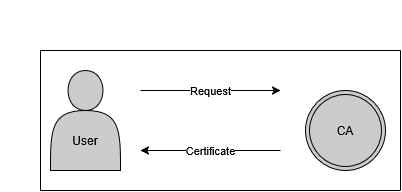
\includegraphics[scale=0.7]{figure1.png}
\caption{Diagram of the Certificate Authority (CA) issuing and validating a digital certificate for a user.}
\end{figure}
\paragraph{Explanation}

This diagram illustrates the process of certificate issuance and verification in the Public Key Infrastructure (PKI) model.

First, the user submits their identity and RSA public key components $(n,e)$ to the Certificate Authority (CA). The CA constructs a certificate by concatenating the user's identity with the public key values and computing a cryptographic hash over this data.

The CA then signs the hash using its private RSA key, producing a digital signature that binds the user's identity to their public key. The final certificate consists of the tuple $(ID, n, e, \text{Signature})$.

Any party can later verify the authenticity of the certificate using the CA's public key. If the verification succeeds, the public key is considered trustworthy.


\subsection{Authenticated Diffie-Hellman Key Exchange}

\begin{figure}[H]
\centering
% 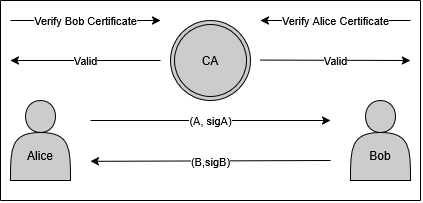
\includegraphics[scale=0.75]{figure2.png}
\caption{Diagram of the authenticated Diffie-Hellman key exchange using RSA-based digital signatures and certificate validation.}
\end{figure}
\paragraph{Explanation}

This diagram shows the authenticated Diffie-Hellman key exchange protocol, which combines symmetric key agreement with public-key authentication.

Before initiating the key exchange, both parties verify each other's certificates using the trusted Certificate Authority (CA). This ensures that the public keys used in the protocol are authentic.

After successful verification, Alice and Bob independently generate private random exponents $a$ and $b$. They compute their public Diffie--Hellman values as $A = g^a \bmod p$ and $B = g^b \bmod p$.

To prevent Man-in-the-Middle attacks, both values are digitally signed using RSA signatures. The signed values are exchanged and verified using the certified public keys.

Finally, both parties compute the shared secret:
\[
K = g^{ab} \bmod p.
\]

Since both computations yield the same result, a secure shared key is established.

%%%%%%%%%%%%%%%%%%%%%%%%%%%%%%%%%%%%%%%%%%%%
%%%%%%%%%%%%%%%%%%%%%%%%%%%%%%%%%%%%%%%%%%%%
\newpage
\section{Experimental Results}

\subsection{End-to-End Execution of the Authenticated Diffie--Hellman Protocol}

To evaluate the correctness and security of the implemented system, a complete
execution scenario involving a Certificate Authority (CA), Alice, and Bob was performed.

The following output demonstrates the step-by-step execution of the protocol:

\begin{lstlisting}[style=console]

=== Diffie-Hellman Authenticated Protocol Start ===

Verifying certificate of A...
A certificate VALID

Verifying certificate of B...
B certificate VALID

Private values generated:
a (Alice secret) generated
b (Bob secret) generated

Public values computed:
A_pub = g^a mod p = 49799
B_pub = g^b mod p = 20312

Digital signatures created:
Alice signs A_pub
Bob signs B_pub

Verifying Alice signature...
Alice signature VALID

Verifying Bob signature...
Bob signature VALID

Computing shared secret...

Shared key computed successfully:
K_A = 44619
K_B = 44619

*** PROTOCOL SUCCESSFUL ***
Secure shared secret established.
K = 44619

\end{lstlisting}

\subsection{Result Analysis}

The experimental results confirm the correctness of the implemented authenticated
Diffie-Hellman protocol.

Both participants independently compute the same shared secret value:

\begin{equation}
K_A = K_B = g^{ab} \bmod p
\end{equation}

This demonstrates that the Diffie--Hellman key exchange works correctly.

Furthermore, all certificates are successfully verified by the Certificate Authority,
and all RSA signatures are validated before key computation.

This ensures that:

\begin{itemize}
\item The communicating parties are authenticated.
\item The exchanged Diffie-Hellman values are not tampered with.
\item The system is resistant to Man-in-the-Middle attacks under the assumed model.
\end{itemize}

Therefore, the implementation successfully achieves both confidentiality and authentication.



%%%%%%%%%%%%%%%%%%%%%%%%%%%%%%%%%%%%%%%%%% KB %%%%%%%%%%%%%%%%%%%%%%%%%%%%%%%%%%%%%%%%%%%%


\section{Feistel-Based Symmetric Encryption System}

\subsection{Purpose}

After the authenticated Diffie--Hellman protocol establishes a shared secret key, a symmetric encryption algorithm is required to provide message confidentiality.

The project implements a custom Feistel-based block cipher that uses the shared master key generated during the authenticated Diffie--Hellman phase. The cipher encrypts plaintext messages before transmission and decrypts them at the receiver side.

The implementation follows all requirements specified in the project description, including 16-bit blocks, four Feistel rounds, round-key generation, S-Box substitution, bit permutation, and ISO/IEC 7816-4 padding.

\subsection{Feistel Network Structure}

\subsubsection{Block Configuration}

The cipher operates on 16-bit blocks:

[
BlockSize = 16 \text{ bits}
]

Each block is divided into:

\begin{itemize}
\item Left Half (L): 8 bits
\item Right Half (R): 8 bits
\end{itemize}

The encryption process consists of four Feistel rounds.

\subsubsection{Mathematical Foundation}

For round $i$:

\[
L_{i+1}=R_i
\]

\[
R_{i+1}=L_i \oplus F(R_i,K_i)
\]

where:

\begin{itemize}
\item $L_i$ and $R_i$ represent the left and right halves,
\item $K_i$ denotes the round key,
\item $F$ denotes the round function.
\end{itemize}

After the final round, the resulting halves are concatenated to produce the ciphertext block.

\subsubsection{Correctness}

One of the main advantages of the Feistel structure is that decryption uses the same algorithm as encryption, with the only difference being that round keys are applied in reverse order.

Therefore, the original plaintext can always be recovered correctly.

\subsection{Round Function $F$}

\subsubsection{Purpose}

The round function introduces confusion and diffusion into the cipher.

\subsubsection{XOR with Round Key}

Given the right half $R$ and round key $K$:

\[
X = R \oplus K
\]

This operation incorporates the secret key into the encryption process.

\subsubsection{S-Box Substitution}

The resulting byte is separated into two 4-bit halves:

\[
HighNibble = X >> 4
\]

\[
LowNibble = X \mathbin{\&} 0x0F
\]

Each nibble is transformed using the project S-Box shown in Table~\ref{tab:sbox}.

\begin{table}[h]
\centering
\caption{S-Box Used in the Feistel Cipher}
\label{tab:sbox}
\begin{tabular}{|c|c|}
\hline
Input & Output \\
\hline
0 & 12 \\
1 & 5 \\
2 & 6 \\
3 & 11 \\
4 & 9 \\
5 & 0 \\
6 & 10 \\
7 & 13 \\
8 & 3 \\
9 & 14 \\
10 & 15 \\
11 & 8 \\
12 & 4 \\
13 & 7 \\
14 & 1 \\
15 & 2 \\
\hline
\end{tabular}
\end{table}

The S-Box introduces non-linearity and increases resistance against simple cryptanalytic attacks.

\subsubsection{Bit Permutation}

After substitution, the bits are permuted according to:

\[
P = [0, 4, 2, 6, 1, 5, 3, 7]
\]

The permutation spreads local changes throughout the output and improves diffusion.

\subsubsection{Security Contribution}

The combination of:

\begin{enumerate}
\item XOR key mixing
\item Non-linear substitution
\item Bit permutation
\end{enumerate}

provides the essential cryptographic properties required for block cipher design.

\subsection{Round Key Generation}

\subsubsection{Purpose}

Each Feistel round requires a distinct round key derived from the shared master key.

\subsubsection{Mathematical Foundation}

Let $K$ denote the 16-bit master key obtained from the authenticated Diffie--Hellman protocol.

Round key $i$ is generated as:

\[
K_i = \left( (K \gg i) \oplus (K \gg (i+4)) \right) \mathbin{\&} 0xFF
\]

for:

\[
i \in \{1,2,3,4\}
\]

\subsubsection{Implementation}

The implementation derives four independent 8-bit round keys.

Using different round keys ensures that each Feistel round performs a different transformation.

\subsection{Message Encoding}

\subsubsection{ASCII Conversion}

User messages are initially represented as character strings.

Each character is converted to its ASCII value and then represented as an 8-bit binary sequence.

Example:

[
'H' = 72 = 01001000
]

[
'i' = 105 = 01101001
]

The resulting binary sequences are concatenated into a single bit stream.

\subsubsection{Block Formation}

The bit stream is divided into consecutive 16-bit blocks before encryption.

Each block is processed independently by the Feistel cipher.

\subsection{ISO/IEC 7816-4 Padding}

\subsubsection{Purpose}

Since the message length may not be an exact multiple of the block size, padding is required.

\subsubsection{Padding Procedure}

The implementation follows ISO/IEC 7816-4.

The procedure is:

\begin{enumerate}
\item Append byte $10000000$.
\item Append zero bytes until the total length becomes a multiple of 16 bits.
\end{enumerate}

Padding is always added, even when the original message length already aligns perfectly with the block boundary.

\subsubsection{Example}

Message:

\texttt{Hi}

Binary representation:

[
01001000 \ 01101001
]

Padding:

[
10000000 \ 00000000
]

Final blocks:

[
0100100001101001
]

[
1000000000000000
]

\subsubsection{Padding Removal}

During decryption:

\begin{enumerate}
\item The binary stream is reconstructed.
\item Trailing zero bytes are removed.
\item The first encountered byte equal to $10000000$ is removed.
\item The original plaintext message is recovered.
\end{enumerate}

\subsection{Security Analysis}

The implemented cipher is intended for educational purposes and demonstrates the principles of modern block cipher design.

The cipher provides:

\begin{itemize}
\item Key-dependent transformations
\item Multiple encryption rounds
\item Non-linear substitution
\item Bit-level diffusion
\end{itemize}

However, it should not be considered secure for real-world deployment because:

\begin{itemize}
\item The block size is only 16 bits.
\item The key size is only 16 bits.
\item The number of rounds is limited.
\item Modern block ciphers employ significantly stronger designs.
\end{itemize}

Despite these limitations, the implementation successfully demonstrates the core concepts of symmetric cryptography.

\subsection{Experimental Results}

\subsubsection{Encryption Test}

After the authenticated Diffie--Hellman protocol generated the shared master key, a plaintext message was encrypted using the Feistel cipher.

Example message:

\texttt{Hello TA}

The message was converted into binary form, padded using ISO/IEC 7816-4, divided into 16-bit blocks, and encrypted successfully.

The program produced a sequence of encrypted integer blocks.

\subsubsection{Decryption Test}

The encrypted blocks were supplied to the decryption module.

After applying Feistel decryption, removing padding, and converting the recovered binary stream back into ASCII characters, the original plaintext message was reconstructed successfully.

\subsubsection{Result Analysis}

The experimental results confirm that:

\begin{itemize}
\item Binary encoding functions correctly.
\item ISO/IEC 7816-4 padding is applied and removed correctly.
\item Feistel encryption and decryption operate correctly.
\item The original plaintext is recovered without loss of information.
\item The shared key generated during the authenticated Diffie--Hellman protocol is successfully used as the symmetric encryption key.
\end{itemize}

Therefore, the implementation successfully fulfills all Phase 3 requirements of the project and completes the secure messaging system.


\section{User Interface and System Integration}

\subsection{Purpose}

The final phase of the project focuses on integrating all cryptographic components into a single interactive application.

The objective of the user interface is to provide a simple mechanism for executing the complete secure communication workflow while hiding implementation details from the user.

The interface connects the following components:

\begin{itemize}
\item RSA Key Generation
\item Certificate Authority (CA)
\item Certificate Verification
\item Authenticated Diffie--Hellman Key Exchange
\item Feistel Encryption
\item Feistel Decryption
\end{itemize}

All components are executed within a single Java application.

\subsection{System Architecture}

The implementation follows a modular architecture consisting of multiple packages:

\begin{itemize}
\item \texttt{phase1} -- RSA, PKI, and Certificate Management
\item \texttt{phase2} -- Authenticated Diffie--Hellman
\item \texttt{phase3} -- Feistel Cipher and Padding
\item \texttt{app} -- Integration and Application State Management
\item \texttt{ui} -- Console-Based User Interface
\end{itemize}

This design separates cryptographic functionality from user interaction and improves maintainability.

\subsection{Application State Management}

A dedicated application state object stores the current system status.

The stored information includes:

\begin{itemize}
\item CA Public Key
\item User A Public Key
\item User B Public Key
\item User Certificates
\item Certificate Verification Status
\item Shared Master Key
\item Last Encrypted Message Blocks
\end{itemize}

This approach allows different menu operations to access previously generated cryptographic data.

\subsection{Menu Structure}

The application provides a console-based menu consisting of six options.

\begin{enumerate}
\item Initialize System
\item Establish Shared Key
\item Encrypt Message
\item Decrypt Message
\item Show Current Status
\item Exit
\end{enumerate}

The menu remains active until the user chooses the exit option.

\subsection{Initialize System}

The first menu option performs the initialization phase.

The following operations are executed:

\begin{enumerate}
\item Generate the CA RSA key pair.
\item Generate User A RSA key pair.
\item Generate User B RSA key pair.
\item Issue certificates for both users.
\item Verify generated certificates.
\item Store all public information in the application state.
\end{enumerate}

Successful completion of this phase indicates that the PKI infrastructure has been established.

\subsection{Establish Shared Key}

The second menu option executes the authenticated Diffie--Hellman protocol.

The following operations are performed:

\begin{enumerate}
\item Validate both certificates.
\item Generate Diffie--Hellman private values.
\item Compute public Diffie--Hellman values.
\item Generate RSA signatures.
\item Verify signatures.
\item Compute the shared secret.
\item Derive the 16-bit master key.
\end{enumerate}

The generated master key becomes the symmetric key used by the Feistel cipher.

\subsection{Message Encryption}

The third menu option encrypts a plaintext message.

The workflow is:

\begin{enumerate}
\item Receive plaintext input from the user.
\item Convert characters to ASCII binary representation.
\item Apply ISO/IEC 7816-4 padding.
\item Divide the message into 16-bit blocks.
\item Encrypt each block using the Feistel network.
\item Display encrypted blocks.
\item Store encrypted blocks for future decryption.
\end{enumerate}

\subsection{Message Decryption}

The fourth menu option decrypts encrypted message blocks.

The workflow is:

\begin{enumerate}
\item Receive encrypted blocks.
\item Apply Feistel decryption.
\item Reconstruct the binary stream.
\item Remove ISO/IEC 7816-4 padding.
\item Convert ASCII values back to characters.
\item Display the recovered plaintext.
\end{enumerate}

Successful execution demonstrates the correctness of the implemented symmetric cipher.

\subsection{Status Monitoring}

The fifth menu option displays the current system status.

The following information is shown:

\begin{itemize}
\item CA Public Key
\item User A Public Key
\item User B Public Key
\item Certificate Verification Status
\item Current Master Key
\item Last Encrypted Ciphertext
\end{itemize}

This functionality assists in debugging and validating the protocol execution.

\subsection{Experimental Demonstration}

A complete end-to-end execution was performed using the integrated user interface.

The following sequence was executed:

\begin{enumerate}
\item Initialize System
\item Establish Shared Key
\item Encrypt Message
\item Decrypt Message
\item Display Current Status
\end{enumerate}

The execution confirmed that:

\begin{itemize}
\item Certificates are generated and verified successfully.
\item The authenticated Diffie--Hellman protocol establishes a valid shared secret.
\item The Feistel cipher encrypts plaintext correctly.
\item The decryption process recovers the original message.
\item All components operate correctly within a single integrated application.
\end{itemize}

\subsection{Conclusion}

The final integrated application successfully combines public-key cryptography, certificate management, authenticated key exchange, and symmetric encryption into a single secure messaging system.

The user interface provides a convenient mechanism for executing the entire protocol while maintaining a modular software architecture.

Therefore, the project satisfies all functional requirements described in the assignment specification.


\end{document}